\documentclass{acm_proc_article-sp}
\begin{document}

\title{Creepture: Virtual Caterpillar-like Robot that Achieves Locomotion
Automatically through Evolutionary Computation}

\numberofauthors{1}
\author{
    \alignauthor
    Rob Murrer \\ 
    \affaddr{University of Central Florida}\\
        \email{c@robmurrer.com}
   }

\date{10 April 2014}

\maketitle
\begin{abstract}
This paper presents an Evolutionary Computation approach to automatically
realize locomotion with a modular virtual caterpillar-like robot called
Creepture. Without any prior intelligence besides the number of modules
available, a Genetic Algorithm (GA) optimizes a network of Central
Pattern Generators that are connected to each joint in the Creepture.
This was accomplished through a simulation layer in the fitness function
of the GA. Successful locomotion in a desired direction was realized for
Creeptures with up to 4 modules.
\end{abstract}

\terms{Evolutionary Computation, Genetic Algorithm, Central Pattern Generator}

\section{Introduction}
Locomotion is an essential behavior of most organisms. How the
locomotive patterns are acquired for efficient movement can be thought
of intuitively as a trial-and-error feedback loop. A child learning to
crawl will attempt many times and fail before they are able to move in a
desired manner. Because this process can be thought of as an
optimization, Evolutionary Computation (EC) and specifically Genetic
Algorithms (GAs) have been used to create automatic locomotion {[}1{]}
{[}2{]}.

Through a network of Central Pattern Generators (CPGs), a locomotive
pattern is created. These CPGs create non-linear oscillations that
excite or inhibit muscle movement. The network of CPGs work in concert
to create complex movement such as locomotion. The parameters of a CPG
network increase exponentially as the network increases. Because the
number of parameters can be so large, creating desired movements is
increasing difficult as the number of modules increase.

The EC approach using a GA to optimize the CPG network was used to
achieve semi-realistic caterpillar-like movement. A simulation layer was
created using the \emph{Box2D} physics engine and was used in the
fitness function within the GA. The segments of the Creepture are similar
to the \emph{M-TRAN} modules created by Kimura et al {[}1{]}. These
segments are fused together and locomotion was realized on Creeptures up
to 4 segments.

\section{The Creepture System}
A network of CPGs was created to drive the Creepture modules. Two CPGs
are required per module. The modules were modeled in the \emph{Box2D}
physics engine and connected to the CPG network. Parameters of the CPG
network were then optimized by the GA according to the distance and
energy used as computed from \emph{Box2D} simulation.

\subsection{Central Pattern Generator}

CPGs are non-traditional artificial neural networks.  Each CPG controls
one joint motor within a Creepture segment. There are four neurons within
each CPG that operate in pairs to control the extensor and flexor
movements of the joint. As can be seen in Figure \ref{cpgpic},
connections be either excitatory or inhibitory.

\begin{figure}
\centering
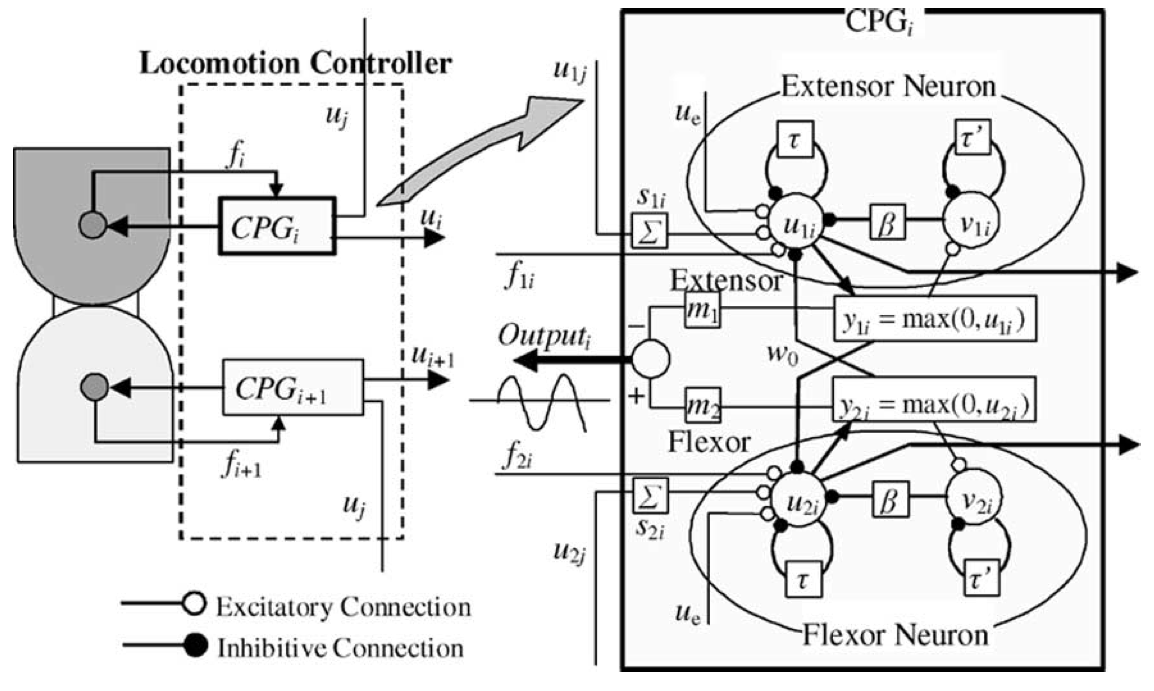
\includegraphics[width=0.5\textwidth]{images/cpg.png}
\caption{M-Tran module and Central Pattern Generator [1] \label{cpgpic}}
\end{figure}

CPGs placed in a network were connected with discrete weights values:
\texttt{-1} inhibitory, \texttt{0} no connection, and \texttt{1}
excitatory. There are also four state variables associated with the
values of the neurons in the CPG $(u_{1i}, v_{1i}, u_{2i}, v_{2i})$.
These neuron states can take on continuous values from -1.0 to 1.0. The
equations (1) and (2) are used to model a CPG network.

\begin{multline}
\begin{aligned}
    &\begin{cases}
        \tau\dot{u}_{1j} = -u_{1j} - w_{0}y_{2i} - \beta v_{1i} + u_e + s_{1i} \\
        \tau'\dot{v}_{1i} = -v_{1i} + y_{1i}
    \end{cases}
    \\
    &y_{1i} = max(0, u_{1i}), i = 0,...,num-1
\end{aligned}
\end{multline}

\begin{multline}
\begin{aligned}
    &\begin{cases}
        \tau\dot{u}_{2j} = -u_{2j} - w_{0}y_{1i} - \beta v_{2i} + u_e + s_{2i} \\
        \tau'\dot{v}_{2i} = -v_{2i} + y_{2i}
    \end{cases}
    \\
    &y_{2i} = max(0, u_{2i}), i = 0,...,num-1
\end{aligned}
\end{multline}

The subscripts of 1 and 2 represent the extensor and flexor neuron pairs within the CPG, and the num
represents the number of joints present in the network.  The variables
$s_1$ and $s_2$ are the weighted connections to the rest of the network
and are defined in equations (3) and (4). The variable $s$ is normalized
between -1.0 and 1.0 via the sigmoid function.

\begin{multline}
\begin{aligned}
    s_{1i} &= 2.0 *  \left\{1 + \text{exp}\left(\frac{-\text{feed}_{1i}}{\text{num}}\right)\right\}^{-1} - 1.0 \\ 
    \text{feed}_{1i} &= \sum_j \text{weight}_{ij}u_{1j}
\end{aligned}
\end{multline}

\begin{multline}
\begin{aligned}
    s_{2i} &= 2.0 *  \left\{1 + \text{exp}\left(\frac{-\text{feed}_{2i}}{\text{num}}\right)\right\}^{-1} - 1.0 \\ 
    \text{feed}_{2i} &= \sum_j \text{weight}_{ij}u_{2j}
\end{aligned}
\end{multline}

The CPG drives the Creepture module in the simulation through
controlling motor speed and direction. The speed is calculated by
equation (5). In electrical engineering parlance this could be thought
of as voltage provided to the joint motor. The only difference between
this CPG model and the one used in {[}2{]} is the absence of a feedback
mechanism for the joint angle. This was eliminated because the Creepture
modules always start in the same orientation and the variable was
non-contributory.

\begin{equation}
    \text{Output}_{i} = -m_1 y_{1i} + m_2 y_{2i} 
\end{equation}

There are many constant parameters in the CPG that are not optimized by
the GA. These values were initially taken from {[}1{]} and adjusted
through experimentation to achieve results suitable for the Creepture
module (Table 1).

\begin{table}
\centering
\caption{CPG Constant Parameters}
\begin{tabular}{|l|l|} \hline
Parameter & Value\\ \hline
$\tau$ & 0.6\\ \hline
$\tau`$ & 0.6\\ \hline
$\beta$ & 5.5\\ \hline
$w_0$ & 2.0\\ \hline
$u_e$ & 1.0\\ \hline
$m_1, m_2$ & 700.0\\ \hline
\end{tabular}
\end{table}

\subsection{Creepture Module}

Each module or segment of the Creepture can be seen in Figure 2. The
segment was modeled after \emph{M-TRAN} module {[}1{]}. Segments are
composed of two circles and a thin rectangle. The two circles are pinned
to the bar through two \emph{Revolute} joints in the \emph{Box2D} world.
These joint have motors attached to them and are driven individually by
a CPG.

\begin{figure}
\centering
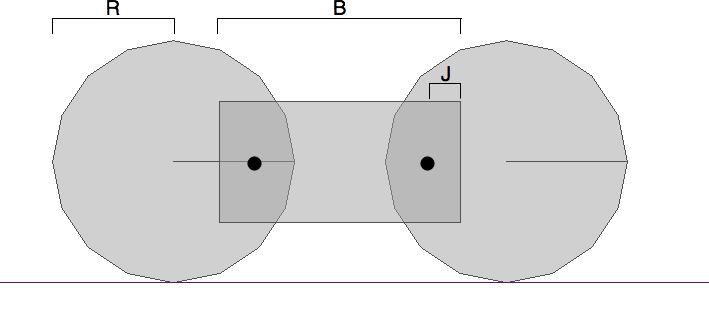
\includegraphics[width=0.5\textwidth]{images/segment-annotated.png}
\caption{Creepture Segment, Box2D measurements: R:2.0, B:4.0, J:1.0. Max
Joint Angle: $\pm$ 90.0$\deg$ \label{creepturemod}}
\end{figure}

The number of modules of the Creepture can be varied before the start of
a GA run. Each module is fused together with the previous module
creating a chain (Figure 3).

\subsection{Genetic Algorithm}\label{genetic-algorithm}

A GA was created for optimization of variable parameters within the
network of CPGs: weights between CPGs and initial neuron states
$(u_1(0), v_1(0), u_2(0), v_2(0))$. These parameters were optimized to
create the most efficient form of locomotion in a single direction
(right).

\begin{table}
\centering
\caption{Genetic Algorithm Parameters}
\begin{tabular}{|l|l|} \hline
Parameter & Value\\ \hline
pop\_size & 100\\ \hline
max\_gene & 150\\ \hline
elites & 30\\ \hline
xover\_rate & 0.7\\ \hline
mut\_rate & 0.05\\ \hline
\end{tabular}
\end{table}

\subsubsection{Fitness}

At each generation the members of the population went through a
simulation within the physics engine. This was done by approximating
each CPGs state through equations (1) and (2) using the \emph{Euler}
method. The output of each CPG was then connected through equation (5)
to a joint motor within the simulation; this was done at each tick or step in the
simulation. Each member of the population was simulated for 20 seconds.

\begin{equation}
    \text{fitness} = \text{distance} - \gamma \frac{\text{energy}}{\text{num}}
\end{equation}

The fitness of an individual is then calculated using (6) where distance in the "correct" direction is assessed.
The energy expended in the simulation is then divided by the number of modules and
multiplied by constant $\gamma$ of value 0.01. This is then subtracted from
the distance in order to encourage efficient locomotion.

\subsubsection{Selection and Mutation}

Elites in the population are not mutated and remain unchanged during a
single generation. They are used in a random crossover with the rest of
the population and an N-Point crossover occurs in accordance to the
\emph{xover\_rate} in Table 2.

After the crossover stage of the GA, mutation occurs to the members who
were affected. The \emph{mut\_rate} dictates the probability in which a
gene will be mutated. For the discrete values of the weights between the
CPGs in the network, a random value was chosen (-1, 0, 1). The initial
values of the neurons in the CPGs are continuous so they were mutated
based on a range of $\pm 0.01$ making sure the values never exceeded the
bounds of -1.0 to 1.0.

\subsection{Procedure for testing}

To evaluate the effectiveness of the Creepture system and to determine
the upper limit on the number of modules, the following procedure was used.

\begin{enumerate}
\itemsep1pt\parskip0pt\parsep0pt
\item
  Set segment count starting at 2
\item
  Run GA with this number of segments 3 times.
\item
  Average the distances of the best individual from each run at 20s,
  40s, 60s (Table 3)
\item
  Increase module count by 1 until 5 modules are tested.
\item
  Goto Step 2.
\end{enumerate}

\section{Results}

Locomotion was realized for all Creeptures containing up to 5 segments.
As the segment count was increased the distance of movement after 40s
declined. By limiting the number of segments a Creepture had a more
stable locomotion pattern over time. 

\begin{figure}
\centering
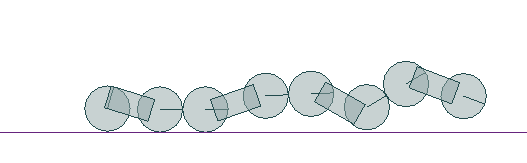
\includegraphics[width=.5\textwidth]{images/chain.png}
\caption{5 Segment Creepture in Action \label{chain}}
\end{figure}

\begin{table}
\centering
\caption{Average Distance Traveled for 2-5 Segments}
\begin{tabular}{|l|l|l|l|} \hline
Segments & 20s & 40s & 60s\\ \hline
2 & 58 & 122 & 185\\ \hline
3 & 53 & 110 & 138\\ \hline
4 & 37 & 71 & 119\\ \hline
5 & 37 & 58 & 61\\ \hline
\end{tabular}
\end{table}

\section{Discussion}

Increasing the number of segments in a Creepture had a negative impact on
the performance of the locomotion long term. The complexity of the
movement and the number of variables to be optimized may be too large
for a \texttt{max\_gene} of \texttt{150}. The fitness function also may
be a culprit of the decline in distance after 20s.

In order to keep runtime down on the GA, fitness calculations are
limited to a 20s execution time in the simulation. Even though this is
not a real-time value, increasing this value by 2x will effectively
double the run time of the GA.  A multi-threaded approach may need to be employed to generate sufficient locomotion patterns for Creeptures having greater than 4 segments.

The success of locomotion for extended periods remains unsolved by these experiments and requires more study to create long-term stable locomotion patterns.  Given the Creepture has no feed back mechanism indicating when a segment is on or off the ground appears to be a problem for long-term locomotion and offers an area for future study.  The CPG network initially generates a successful pattern at first but the pace of the Creepture causes a premature stalling of the movement.  This has been witnessed in [2] and these feedback mechanisms may be integrated into the CPGs of future Creeptures.



\section{References}

{[}1{]} Kamimura, A., Kurokawa, H., Yoshida, E., Murata, S., Tomita, K.
and Kokaji, S. 2005. Automatic locomotion design and experiments for a
modular robotic system. \emph{Mechatronics, IEEE/ASME Transactions on}.
10, 3 (June 2005), 314--325.

{[}2{]} Kimura, H., Sakurama, K. and Akiyama, S. 1998. Dynamic walking
and running of the quadruped using neural oscillator. \emph{Intelligent
robots and systems, 1998. proceedings., 1998 iEEE/rSJ international
conference on} (Oct 1998), 50--57 vol.1.

\end{document}
